\section{Applications}

\subsection{Quantifier elimination}
One of the first applications of parametric Gröbner bases was presented by its inventor Weispfenning \cite{Weispfenning} in the original article. It concerns the problem of computing a system of polynomial equations, whose solutions are equivalent to solutions to a set of logical expressions involving polynomial equations, con- and disjunctions, negations and existential quantifiers.

Specifically, we're given a formula $\exists x_{1}, \dots, x_{n} : \phi(U, x_{1}, \dots, x_{n})$ where $\phi$ is a logical formula, which is a combination using $\land$ and $\lor$ of polynomial equalities and inequalities in $k[U, X]$. If $k_{1}$ is an extension field of $k$, then that formula determines a partioning of $k_{1}^{|U|}$, namely those values of $U$ where the formula is true and those where it isn't. Our goal is to find a system of polynomial equations in $k[U]$ that is satisfied in exactly the same points.

First, we need to normalize the logical expressions, to fit a format we can work with.

\begin{definition}[Positive, primitive formula]
  A logical formula $\varphi$ is called \textit{positive and primitive} if it only involves polynomial equalities in $k[X]$, conjunctions and existential quantifiers.
\end{definition}

\begin{lemma}\label{lem:logical_positive}
Let $\phi = \exists x_{1}, \dots, x_{n} : \phi'(U, x_{1}, \dots, x_{n})$ be a logical formula, where $\phi'$ only contains polynomial equalities and inequalities, conjunctions, disjunctions and negations. Then there exists a finite set of positive, primitive formula $\varphi_{1}, \varphi_{2}, \dots, \varphi_{r}$ such that $\phi \iff (\varphi_{1} \lor \dots \lor \varphi_{r})$.
\end{lemma}
\begin{proof}
  First, the following recursive function transforms $\phi'$ into an equivalent logical formula without any negations or inequalities:

  \begin{align*}
    P(f = 0) &\implies f = 0 \\
    P(f \neq 0) &\implies \exists t : f \cdot t - 1 = 0 \\
    P(\neg(f = 0)) &\implies P(f \neq 0) \\
    P(\neg(\neg(\phi_{0}))) &\implies P(\phi_{0}) \\
    P(\neg(\phi_{0} \land \phi_{1})) &\implies P(\neg \phi_{0}) \lor P(\neg \phi_{1}) \\
    P(\neg(\phi_{0} \lor \phi_{1})) &\implies P(\neg \phi_{0}) \land P(\neg \phi_{1}) \\
    P(\phi_{0} \land \phi_{1}) &\implies P(\phi_{0}) \land P(\phi_{1}) \\
    P(\phi_{0} \lor \phi_{1}) &\implies P(\phi_{0}) \lor P(\phi_{1})
  \end{align*}

  The function terminates, since each recursive call is on a strictly smaller expression. Next, the following recursive function moves disjunctions and existential quantifiers to the top of the expression.

  \begin{align*}
    T(f = 0) &\implies f = 0 \\
    T(\phi_{0} \lor \phi_{1}) &\implies T(\phi_{0}) \lor T(\phi_{1}) \\
    T(\exists t : \phi_{0}) &\implies \begin{cases}
                                        (\exists t : \phi_{0}^{0}) \lor \dots \lor (\exists t : \phi_{0}^{n}) & T(\phi_{0}) = \phi_{0}^{0} \lor \phi_{0}^{1} \lor \dots \lor \phi_{0}^{n} \\
                                        \exists t : T(\phi_{0}) & \text{otherwise}
                                      \end{cases} \\
    T(\phi_{0} \land \phi_{1}) &= \implies \begin{cases}
                                             T(\phi_{0}^{0} \land \phi_{1}) \lor T(\phi_{0}^{1} \land \phi_{1}) & T(\phi_{0}) = \phi_{0}^{0} \lor \phi_{0}^{1} \\
                                             T(\phi_{0} \land \phi_{1}^{0}) \lor T(\phi_{0} \land \phi_{1}^{1}) & T(\phi_{1}) = \phi_{1}^{0} \lor \phi_{1}^{1} \\
                                             \exists t : T(\phi_{0}' \land \phi_{1}) & T(\phi_{0}) = \exists t : \phi_{0}' \\
                                             \exists t : T(\phi_{0} \land \phi_{1}') & T(\phi_{1}) = \exists t : \phi_{1}' \\
                                             \phi_{0} \land \phi_{1} & \text{otherwise}
                                           \end{cases}
  \end{align*}

  Again, this terminates since each recursive call is on a strictly smaller expression. The result is a disjunction of positive, primitive formulas.
\end{proof}

Thus we can solve each of the positive, primitive formulas independently, and see if any of them are satisfiable.

\begin{theorem}
  Let $F \subset k[U, X]$ be a finite set of polynomials over an algebraically closed field and let $G$ be a parametric Gröbner basis of $F$. For a polynomial $f \in k[U][X]$, let $C(f) \subset k[U]$ denote the set of coefficients of non-constant terms in $f$. Then \[ \left(\exists x_{1}, \dots, x_{n} : \bigwedge_{f \in F} f(U, x_{1}, \dots, x_{n}) = 0 \right) \iff \bigwedge_{g \in G} \left( g(U, 0, \dots, 0) = 0 \lor \bigvee_{c \in C(g)} c(U) \neq 0 \right)\] in any extension field $k_{1} \supset k$.
\end{theorem}
\begin{proof}
  Let $\alpha \in k_{1}^{|U|}$. Then the question of whether $\exists x_{1}, \dots, x_{n} : \bigwedge_{f \in F} f(U, x_{1}, \dots, x_{n}) = 0$ is satisfied in $U = \alpha$ is equivalent to whether $\langle \sigma_{\alpha}(F) \rangle$ has a common zero, i.e. if $V(\langle \sigma_{\alpha}(F) \rangle) \neq \emptyset$.

  For the first implication, assume $\exists x_{1}, \dots, x_{n} : \bigwedge_{f \in F} f(U, x_{1}, \dots, x_{n}) = 0$ is satisfied at some $\alpha \in k_{1}^{|U|}$. Let $\beta \in k_{1}^{|X|}$ be a vector of $(x_{1}, \dots, x_{n})$ such that $f(\alpha, \beta) = 0$ for all $f \in F$. Then, since all $g \in G$ are also in $\langle F \rangle$, we get $g(\alpha, \beta) = 0 \; \forall g \in G$. Hence, if $g(\alpha, 0, \dots, 0) \neq 0$, then there has to be some non-constant term in $g$, which is also non-zero at $\alpha$.

  For the other implication, assume every $g \in G$ has zero constant term or some non-zero non-constant term, when viewed as a polynomial in $k[U][X]$. Assume for a contradiction that $V(\langle \sigma_{\alpha}(F) \rangle) = \emptyset$. By the weak Nullstellensatz we get that $1 \in \langle \sigma_{\alpha}(F) \rangle$. Since $G$ is a parametric Gröbner basis, there is some $g \in G$ such that $\LT(\sigma_{\alpha}(g)) \mid 1$. Thus $\sigma_{\alpha}(g)$ is a constant polynomial with non-zero constant term, contradicting the assumption.
\end{proof}


















\subsection{Parametric ideal membership \& theorem discovery}\label{sec:ps_div_app}
We can exploit lemma~\ref{lem:ps_rem_unique} to decide membership problems for parametric ideals.

\begin{theorem}
  Let $k_{1} \supset k$ be field, let $I \subset k[U][X]$ be an ideal, and let $\mathcal G = \{(Y_{1}, G_{1}, \dots, (Y_{n}, G_{n}))\}$ be a comprehensive, reduced Gröbner system for $I$. Let $f \in k[U][X]$ and $\alpha \in k_{1}^{|U|}$, then $\sigma_{\alpha}(f) \in \langle \sigma_{\alpha}(I) \rangle$ if and only if there is an $i$ such that $\alpha \in Y_{i}$ and $\sigma_{\alpha}(r) = 0$, where $r$ is a pseudo-remainder of $f$ modulo $G_{i}$.
\end{theorem}
\begin{proof}
  Fix an $\alpha \in k^{|U|}$, and find some $i$ such that $\alpha \in Y_{i}$. This exists since $\mathcal G$ is comprehensive. Let $G_{i} = \{g_{1}, \dots, g_{m}\}$ and let
  \[c f = r + \sum_{j=1}^{m} h_{j} g_{j}\]
  be a pseudo-reduction. Then $\sigma_{\alpha}(f) \in \langle \sigma_{\alpha}(G_{i}) \rangle = \langle \sigma_{\alpha}(I) \rangle$ if and only if $\sigma_{\alpha}(r) = 0$, by lemma~\ref{lem:ps_rem_unique}.
\end{proof}

In this manner, we can determine conditions on when $\sigma_{\alpha}(f) \in \langle \sigma_{\alpha}(I) \rangle$. We simply require $\sigma_{\alpha}(r) = 0$, i.e. $\alpha \in Y_{i} \cap \V(r)$. Do note, that we might need to repeat this for each $Y$ with $\alpha \in Y$.

It is well-known, that standard geometric constructions can be expressed as polynomial ideals. For example, consider a triangle with vertices $A = (0, 0)$, $B = (x_{1}, y_{1})$ and $C = (x_{2}, y_{2})$. Then expressing that the triangle $ABC$ has a right angle in $A$ corresponds to $x_{1} x_{2} + y_{1} y_{2} = 0$. Then the pythagorean theorem $a^{2} + b^{2} = c^{2}$ corresponds to $x_{1}^{2} + y_{1}^{2} + x_{2}^{2} + y_{2}^{2} = (x_{1} - x_{2})^{2} + (y_{1} - y_{2})^{2}$. In algebraic terms, the fact that the pythagorean theorem holds for right triangles, is the statement that
\[x_{1}^{2} + y_{1}^{2} + x_{2}^{2} + y_{2}^{2} - \left((x_{1} - x_{2})^{2} + (y_{1} - y_{2})^{2}\right) \in \sqrt{\langle x_{1} x_{2} + y_{1} y_{2} \rangle} \]
In general, a geometric conclusion $f \in k[X]$ follows from a set of assumptions generating the ideal $I$ if and only if $f \in \sqrt{I}$. Thankfully, $\sqrt{ \langle x_{1} x_{2} + y_{1} y_{2} \rangle } = \langle x_{1} x_{2} + y_{1} y_{2} \rangle$. However, in general, computing the radical of an ideal is quite difficult. We do however have the following theorem.

\begin{theorem}\label{thm:rad}
  Let $I \subset k[X]$ be an ideal, and let $f \in k[X]$. Then $f \in \sqrt{I}$ if and only if $1 \in I + \langle 1 - yf \rangle \in k[X, y]$, where we have added a new variable. This can be checked using Gröbner bases.
\end{theorem}
\begin{proof}
  See chapter 3,  proposition 8 in~\cite{IVA}. Checking whether $1 \in I + \langle 1 - yf \rangle$ can be done by computing a Gröbner basis $G$ of $I + \langle 1 - yf \rangle$, then $1 \in I + \langle 1 - yf \rangle$ if and only if $G$ contains a unit.
\end{proof}

Hence, if we can compute Gröbner bases, we can automatically prove geometric theorem, which is already pretty cool. But parametric Gröbner bases opens the door for even more: automatic theorem discovery. Most conclusions will not be true, given a set of assumptions. However, using reduced Gröbner systems, we can automatically discover sufficient and necessary assumptions that make the conclusion true.

\begin{theorem}
  Let $I \subset K[U][X]$ be an ideal, let $(Y, G)$ be a segment of a reduced Gröbner system for $I$ and let $f \in k[U][X]$. Assume that $r$ is a pseudo-remainder of $f$ modulo $G$ and that $r \in k[U]$. Then $\sigma_{\alpha}(f) \in \sqrt{\langle \sigma_{\alpha}(I) \rangle}$ if and only if $\sigma_{\alpha}(r) = 0$
\end{theorem}
\begin{proof}
  If $\langle \sigma_{\alpha}(I) \rangle = \langle 1 \rangle$, then the conclusion follows immediately. Hence, we assume that $\langle \sigma_{\alpha}(I) \rangle \neq \langle 1 \rangle$.

  Let $r$ be a pseudo-remainder of $f$ modulo $G$. If $\sigma_{\alpha}(r) = 0$, then $\sigma_{\alpha}(f) \in \langle \sigma_{\alpha}(I) \rangle \subset \sqrt{\langle \sigma_{\alpha}(I) \rangle}$. On the other hand, if $\sigma_{\alpha}(f) \in \sqrt{\langle \sigma_{\alpha}(I) \rangle}$, then $\sigma_{\alpha}(r) \in \sqrt{\langle \sigma_{\alpha}(I) \rangle} $. Hence $1 \in \langle \sigma_{\alpha}(I) \rangle + \langle 1 - y \sigma_{\alpha}(r) \rangle$ by theorem~\ref{thm:rad}. Since $r \in k[U]$, $\sigma_{\alpha}(r) \in k$. Since $\langle \sigma_{\alpha}(I) \rangle \neq \langle 1 \rangle$, meaning $\sigma_{\alpha}(G)$ does not contain a unit, and $\LM(1 - y \sigma_{\alpha}(r)) = y$ when $\sigma_{\alpha}(r) \neq 0$, which is relatively prime with every leading monomial in $\langle \sigma_{\alpha}(I) \rangle$, $\sigma_{\alpha}(G) \cup \{1 - y \sigma_{\alpha}(r)\}$ is a Gröbner basis of $\langle \sigma_{\alpha}(I) \rangle + \langle 1 - y \sigma_{\alpha}(r) \rangle$. Hence, $1 \in \langle \sigma_{\alpha}(I) \rangle + \langle 1 - y \sigma_{\alpha}(r) \rangle$ if and only if $\sigma_{\alpha}(r) = 0$.
\end{proof}

We can use this theorem to discover geometric theorems in the complex plane. Let us look at an example from \cite{MONTES20101391}.


\begin{figure}[t]
  \centering
  \begin{subfigure}{0.4\textwidth}
    \centering
    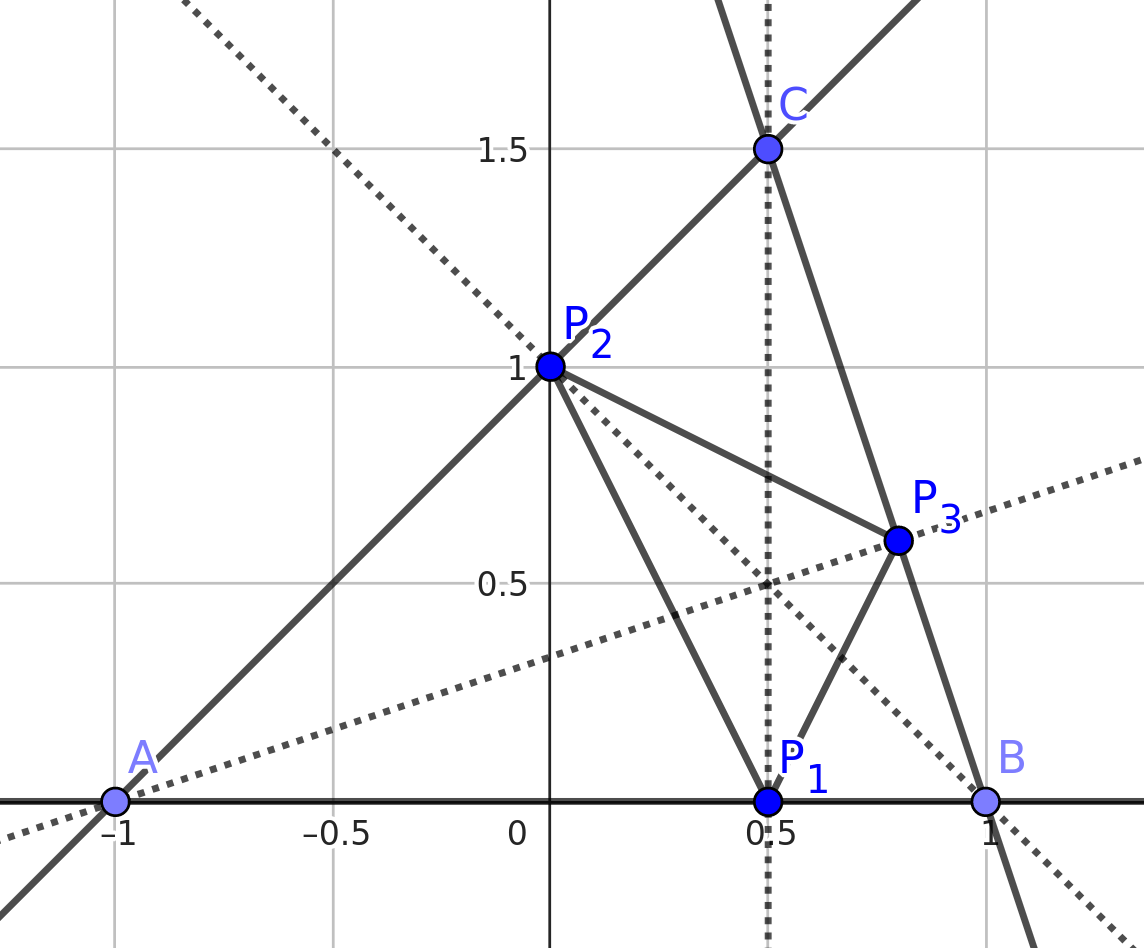
\includegraphics[width=0.9\textwidth]{geogebra_setup.png}
    \caption{A triangle with its orthic triangle drawn.}\label{fig:orthic_setup}
  \end{subfigure}%
  \begin{subfigure}{0.6\textwidth}
    \centering
    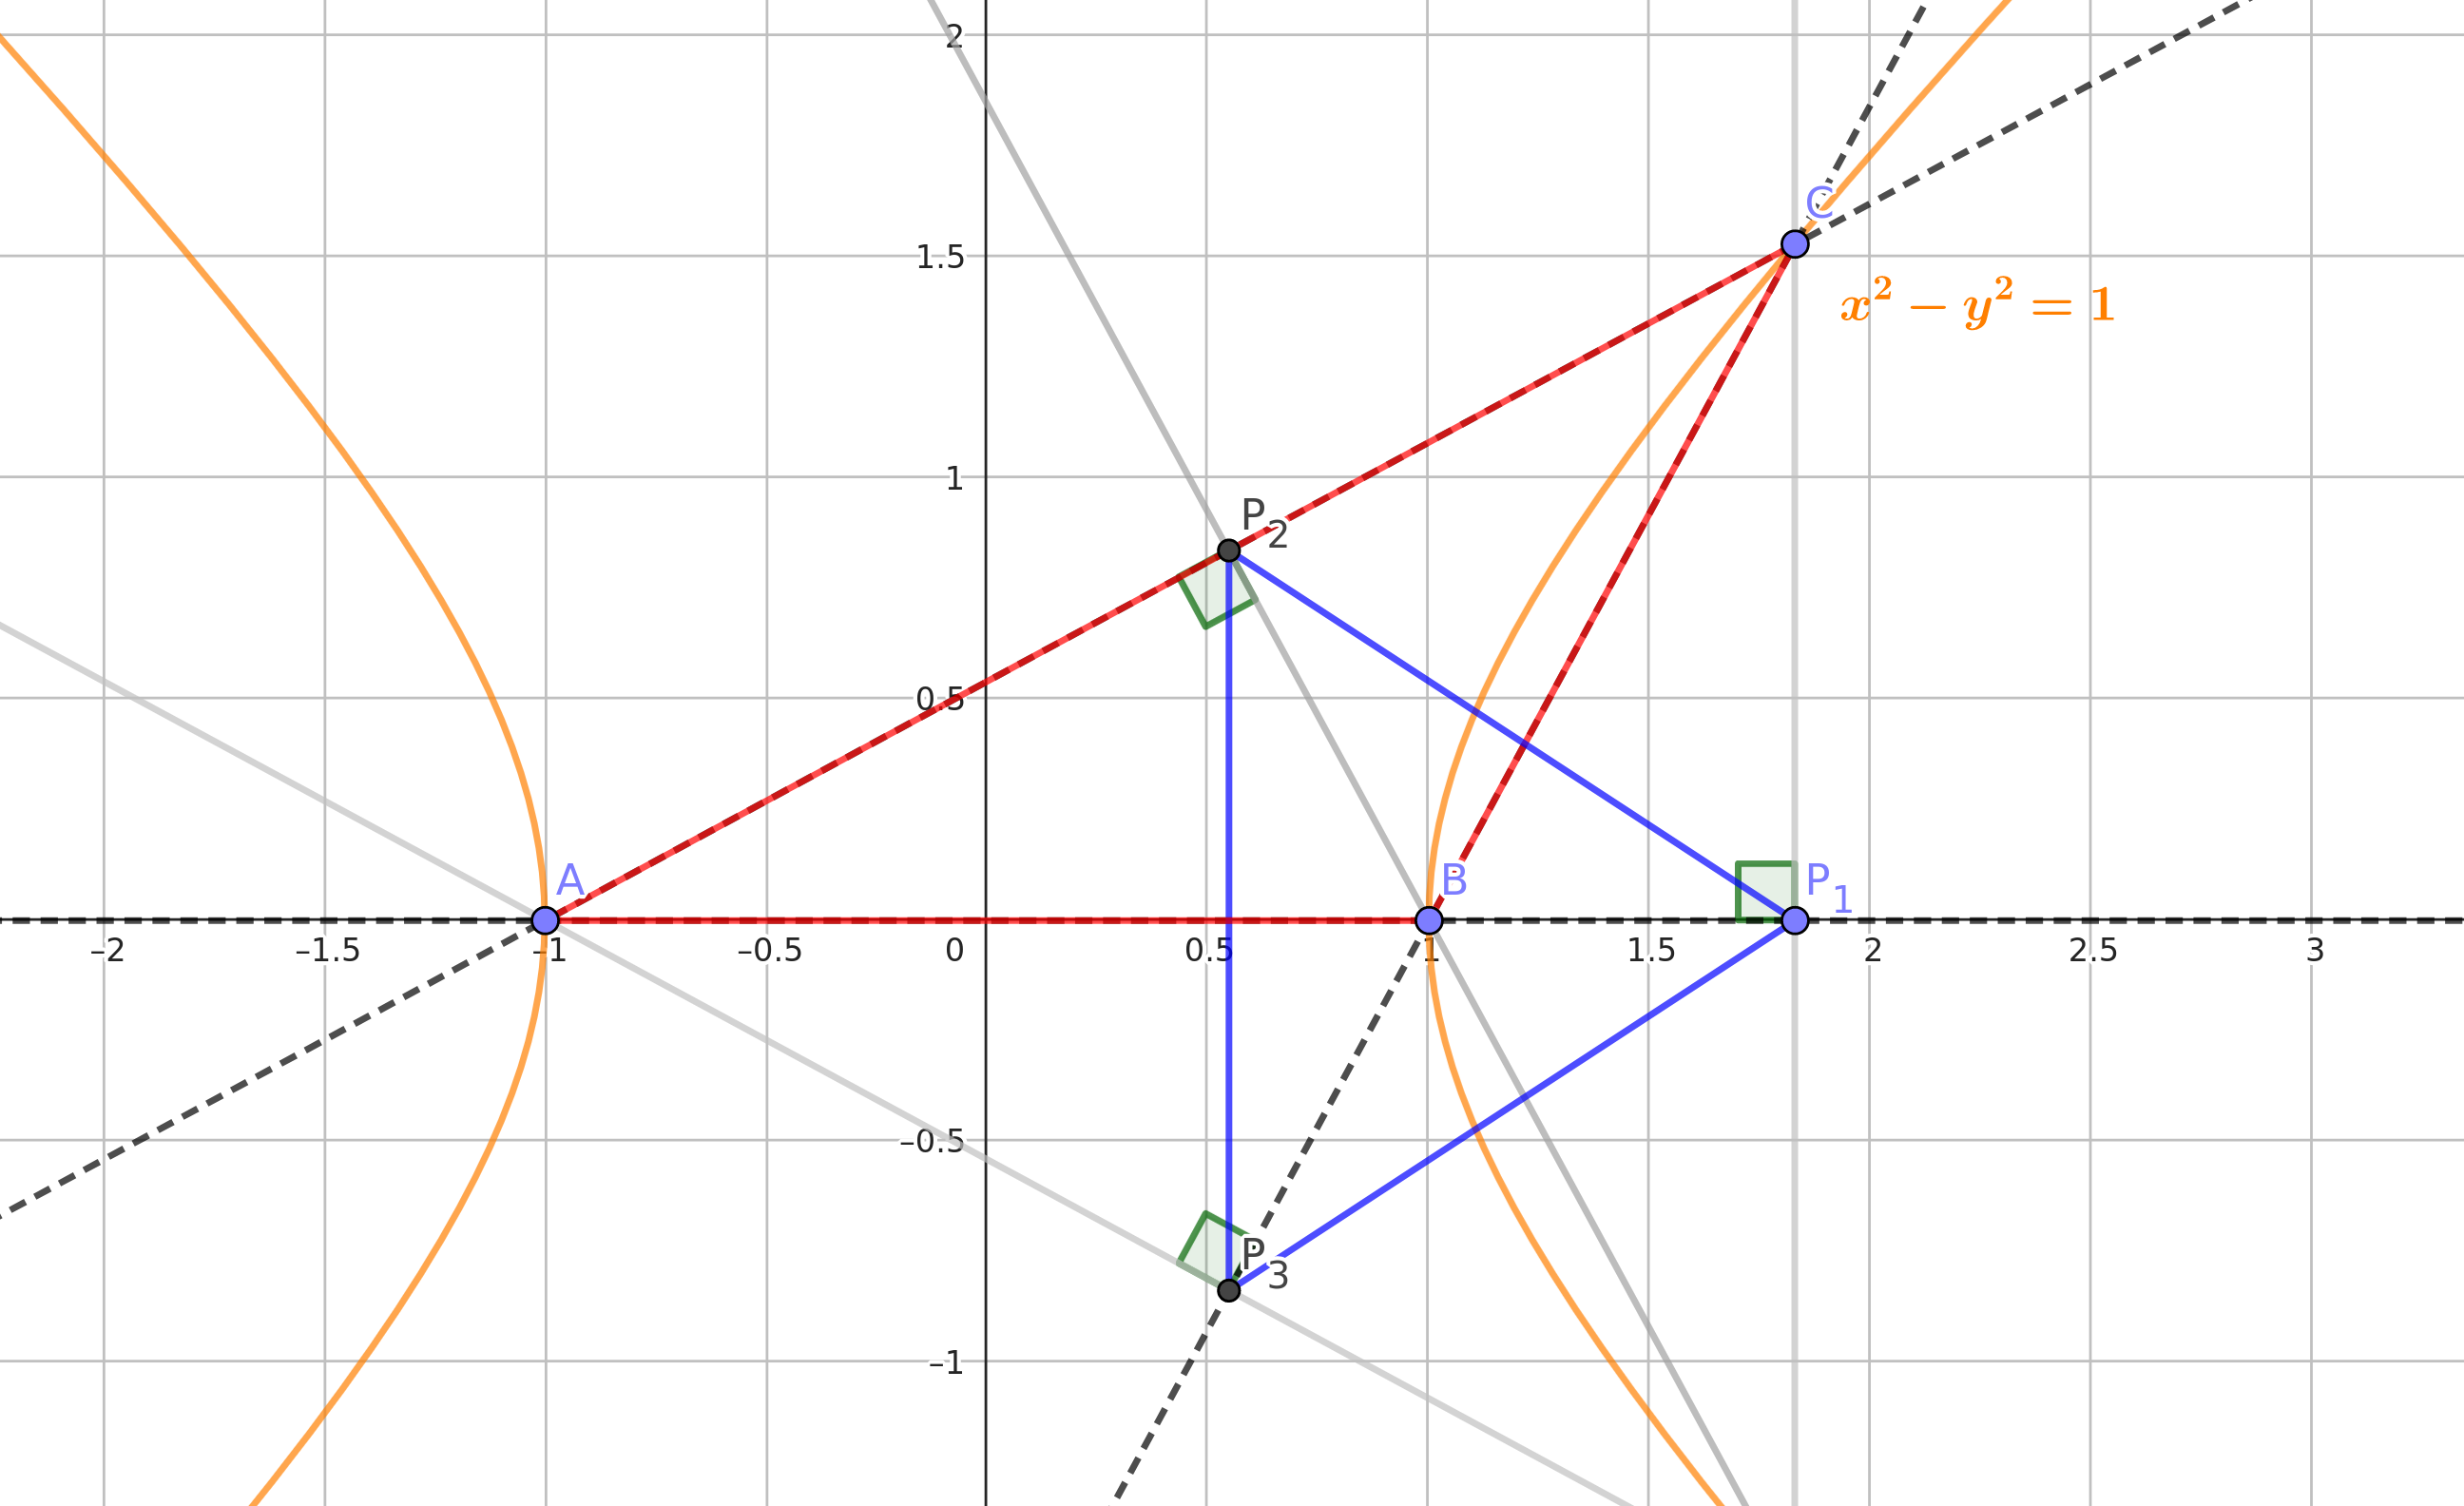
\includegraphics[width=0.9\textwidth]{geogebra_orthic.png}
    \caption{A triangle with a non-obvious isosceles orthic triangle.}\label{fig:orthic_solution}
  \end{subfigure}
  \caption{Orthic triangles}\label{fig:orthic}
\end{figure}

\begin{example} \upshape
  Consider a triangle with vertices $A = (-1, 0)$, $B = (1, 0)$ and $C = (a, b)$. Now, draw the three altitudes of the triangle $ABC$, and label their basepoints $P_{1} = (x_{1}, y_{1})$, $P_{2} = (x_{2}, y_{2})$ and $P_{3} = (x_{3}, y_{3})$, see figure~\ref{fig:orthic_setup}. The triangle $P_{1}P_{2}P_{3}$ is called the \textit{orthic} triangle of $ABC$. We wish to determine when the orthic triangle is isosceles with $|P_{1}P_{2}| = |P_{1}P_{3}|$.

  To solve this problem, we produce a parametric ideal that describes the setup. First, observe that $x_{1} = a$ and $y_{1} = 0$, so we make that substitution immediately. This also ensures that the line $P_{1}C$ is orthogonal to the line $AB$. Next, we need that the line $BP_{2}$ is orthogonal to the line $AC$. This means $0 = BP_{2} \cdot AC = (a + 1)(x_{2} - 1) + b y_{2}$. Similarly, to ensure that $AP_{3}$ is orthogonal to $BC$, we have $0 = (a - 1)(x_{3} + 1) + b y_{3}$. We also need to ensure that the points $P_{2}$ and $P_{3}$ lies on the edges of the triangle. This is done by forcing $0 = b(x_{2} + 1) - (a + 1)y_{2}$ and similarly $0 = b(x_{3} - 1) - (a - 1)y_{3}$. Hence, the following ideal describes the setup:
  \begin{align*}
    I = \langle\; &(a + 1)(x_{2} - 1) + b y_{2}, \quad  b(x_{2} + 1) - (a + 1)y_{2}, \\
                  &(a - 1)(x_{3} + 1) + b y_{3}, \quad  b(x_{3} - 1) - (a - 1)y_{3} \; \rangle
  \end{align*}

  If you want to follow along with the code, here is the setup:
  \begin{minted}{julia}
    using AbstractAlgebra
    using ParametricGrobnerBases
    R, (a, b) = QQ[:a, :b]
    S, (x2, x3, y2, y3) = R[:x2, :x3, :y2, :y3]
    I = [(a + 1)*(x2 - 1) + b*y2, b*(x2 + 1) - (a + 1)*y2, (a - 1)*(x3 + 1) + b*y3, b*(x3 - 1) - (a - 1)*y3]
  \end{minted}

  We want to determine for which values of $a$ and $b$ we have that $\,|P_{1} P_{2}| = |P_{1} P_{3}|$, i.e.\ that $\,0 = f = (x_{3} - a)^{2} + y_{3}^{2} - (x_{2} - a)^{2} + y_{2}^{2}$. This is equivalent to asking whether $\sigma(f) \in \langle \sigma(I) \rangle$ for some specialization $\sigma : \C[a, b] \to \C$.

  \begin{minted}{julia}
    f = (x3 - a)^2 + y3^2 - (x2 - a)^2 - y2^2
  \end{minted}


  To answer this question, we can use the output of $\mathbf{CGS}(I)$. It returns several segments, but most of them has the condition $b = 0$, leading to a degenerate triangle. There is only one case, which is interesting:

  \[V(0) \setminus \V((a^{2} + 2a + b^{2} + 1)(a^{2} - 2a + b^{2} + 1)b)\;, \; G\] where
  \begin{align*}
 G = \{\; &(a^2 - 2a + b^2 + 1)y_3 + 2ab - 2b \\
          &(a^2 + 2a + b^2 + 1)y_2 - 2ab - 2b \\
          &(a^2b - 2ab + b^3 + b)x_3 + a^2b - 2ab - b^3 + b \\
          &(a^2b + 2ab + b^3 + b)x_2 - a^2b - 2ab + b^3 - b \; \}
  \end{align*}

  The condition states that $\sigma(b) \neq 0$. The polynomials $a^{2} + 2a + b^{2} + 1$ and $a^{2} - 2a + b^{2} + 1$ has only the real roots $(a, b) = (-1, 0)$ and $(a, b) = (1, 0)$ respectively. Hence, on the real plane, the condition only states that $\sigma(b) \neq 0$.

  To determine whether $f$ lies in this segment, we compute a pseudo-remainder of $f$ modulo $G$. Like this in Julia:

  \begin{minted}{julia}
    G = CGS(I)[1][3]
    r = pseudo_reduce(f, G)[2]
  \end{minted}
  This gives
  \begin{align*}
    r = &4 a^{17} b^4 + 24 a^{15} b^6 - 32 a^{15} b^4 + 56 a^{13} b^8 - 120 a^{13} b^6 + 112 a^{13} b^4 + 56 a^{11} b^{10} - \\
        &144 a^{11} b^8 + 216 a^{11} b^6 - 224 a^{11} b^4 - 40 a^9 b^{10} + 72 a^9 b^8 - 120 a^9 b^6 + 280 a^9 b^4 - \\
        &56 a^7 b^{14} - 16 a^7 b^{10} + 32 a^7 b^8 - 120 a^7 b^6 - 224 a^7 b^4 - 56 a^5 b^{16} - 72 a^5 b^{14} - \\
        &16 a^5 b^{10} + 72 a^5 b^8 + 216 a^5 b^6 + 112 a^5 b^4 - 24 a^3 b^{18} - 80 a^3 b^{16} - 72 a^3 b^{14} - \\
        &40 a^3 b^{10} - 144 a^3 b^8 - 120 a^3 b^6 - 32 a^3 b^4 - 4 a b^{20} - 24 a b^{18} - 56 a b^{16} - 56 a b^{14} + \\
        &56 a b^{10} + 56 a b^8 + 24 a b^6 + 4 a b^4 \\
    = &4 b^{4}\cdot (a^{2} + 2a + b^{2} + 1)^{3} \cdot (a^{2} - 2a + b^{2} + 1)^{3} \cdot a \cdot (a^{2} - b^{2} - 1) \cdot (a^{2} + b^{2} - 1)
  \end{align*}
  Factorizing multivariate polynomials isn't in Julia yet, unfortunately. It can be done in Macaulay2 or WolframAlpha.

  Since, $\sigma(f) \in \langle \sigma(I) \rangle$ if and only if $\sigma(r) = 0$, we just need to find values of $a$ and $b$, that set $r$ to zero. By considering the factorization, we have five factors, we can make 0, in order to get $r$ to be 0. However, neither $a^{2} + 2a + b^{2} + 1$, $a^{2} - 2a + b^{2} + 1$ nor $b$ can be $0$ by the conditions on the segment. So, we're left with three options.
  \begin{enumerate}
    \item $a = 0$ means that the triangle $ABC$ is isosceles. This immediately gives that $x_{3} = -x_{2}$ and $y_{2} = y_{3}$, which indeed gives us that $|P_{1}P_{2}| = |P_{1}P_{3}|$.
    \item $a^{2} + b^{2} - 1 = 0$ In this case, the triangle has a right angle in vertex $C$, which implies that $P_{2} = P_{3} = C$. Hence, $|P_{1}P_{2}| = |P_{1}P_{3}|$.
          \item $a^{2} - b^{2} - 1 = 0$. This equation traces out a hyperbola, and gives a surprising solution to the problem. Here, the orthic triangle does not sit inside the triangle $ABC$, and the points $P_{1}, P_{2}$ and $P_{3}$ might not be between the vertices. Instead, they lie on the infinite lines described by the vertices. See figure~\ref{fig:orthic_solution}.
  \end{enumerate}

  We also get that for every other value of $a$ and $b$, we have $\sigma(r) \neq 0$ since $\C$ is an integral domain. Hence $\sigma(f) \notin \langle \sigma(I) \rangle$, meaning that the triangle does not have an isosceles orthic triangle. In this way, we have found nescessary and sufficient conditions for the geometric theorem.
\end{example}

It should be noted, that even though the example of finding an isosceles orthic triangle has been worked through in \cite{MONTES20101391}, the method is completely different. In that paper, they computed a Gröbner cover of $I + \langle f \rangle$. While their output is arguably simpler, the method described above has the benefit of being indifferent to the conclusion. In other words, if instead we wanted to ask whether a side of the orthic triangle was parallel to a side of $ABC$, we can do that immediately from $G$ using pseudo-divisions\footnote{The answer is rather boring: it never happens for a non-degenerate triangle.}. In the other approach, we would need to recompute the Gröbner system, which may well take a long time for more complex applications. Let us take one more example, to illustrate why this approach works better in the complex plane than the real plane.

\begin{example}\upshape
  Let $I$ and $G$ be given as before. We want to answer when the area of the orthic triangle is one fifth of the area of the whole triangle. The area of the triangle $ABC$ is $A_{ABC} = b$, and by using the shoelace formula we find that the area of the orthic triangle is $A_{o} = \frac{1}{2}(a(y_{2} - y_{3}) + x_{2} y_{3} - x_{3} y_{2})$. However, those are signed areas, so if the triangle is five times as large as its orthic triangle, we can either have $A_{ABC} = 5 A_{o}$ or $A_{ABC} = -5 A_{o}$. Hence, the polynomial representing the conclusion is $f = (A_{ABC} - 5 A_{o})(A_{ABC} + 5 A_{o})$, since $\sigma(f) = 0$ if either $A_{ABC} = 5 A_{o}$ or $A_{ABC} = -5 A_{o}$. After pseudo-reducing $f$ by $G$, we get a pseudo-remainder that is too large to reproduce, but its factorization is
  \begin{align*}
    r = &-b^{7} \cdot (a^{2} + b^{2} - 2a + 1)^{11} \cdot (a^{2} + b^{2} + 2a + 1)^{8} \cdot \\
        &(11a^{4} + 12a^{2}b^{2} + b^{4} - 22a^{2} - 8b^{2} + 11) \cdot (9a^{4} + 8a^{2}b^{2} - b^{4} - 18a^{2} - 12b^{2} + 9)
  \end{align*}

  We see that $\sigma(f) \in \langle \sigma(I) \rangle$ is and only if $\sigma(11a^{4} + 12a^{2}b^{2} + b^{4} - 22a^{2} - 8b^{2} + 11) = 0$ or $\sigma(9a^{4} + 8a^{2}b^{2} - b^{4} - 18a^{2} - 12b^{2} + 9) = 0$. We'll focus on the first condition. In the complex plane, this is fine. The polynomial is quartic in both $a$ and $b$, so for every fixed $a$-value, we get four solutions for $b$, counted with multiplicity. The real case, however, is not as simple.

  Using a CAS system we get the following roots of the polynomial:
  \[b = \pm \sqrt{4 - 6 a^2 \pm \sqrt{5 - 26 a^2 + 25 a^4}}\]
  We can plot one of the inner functions:

  \begin{center}
    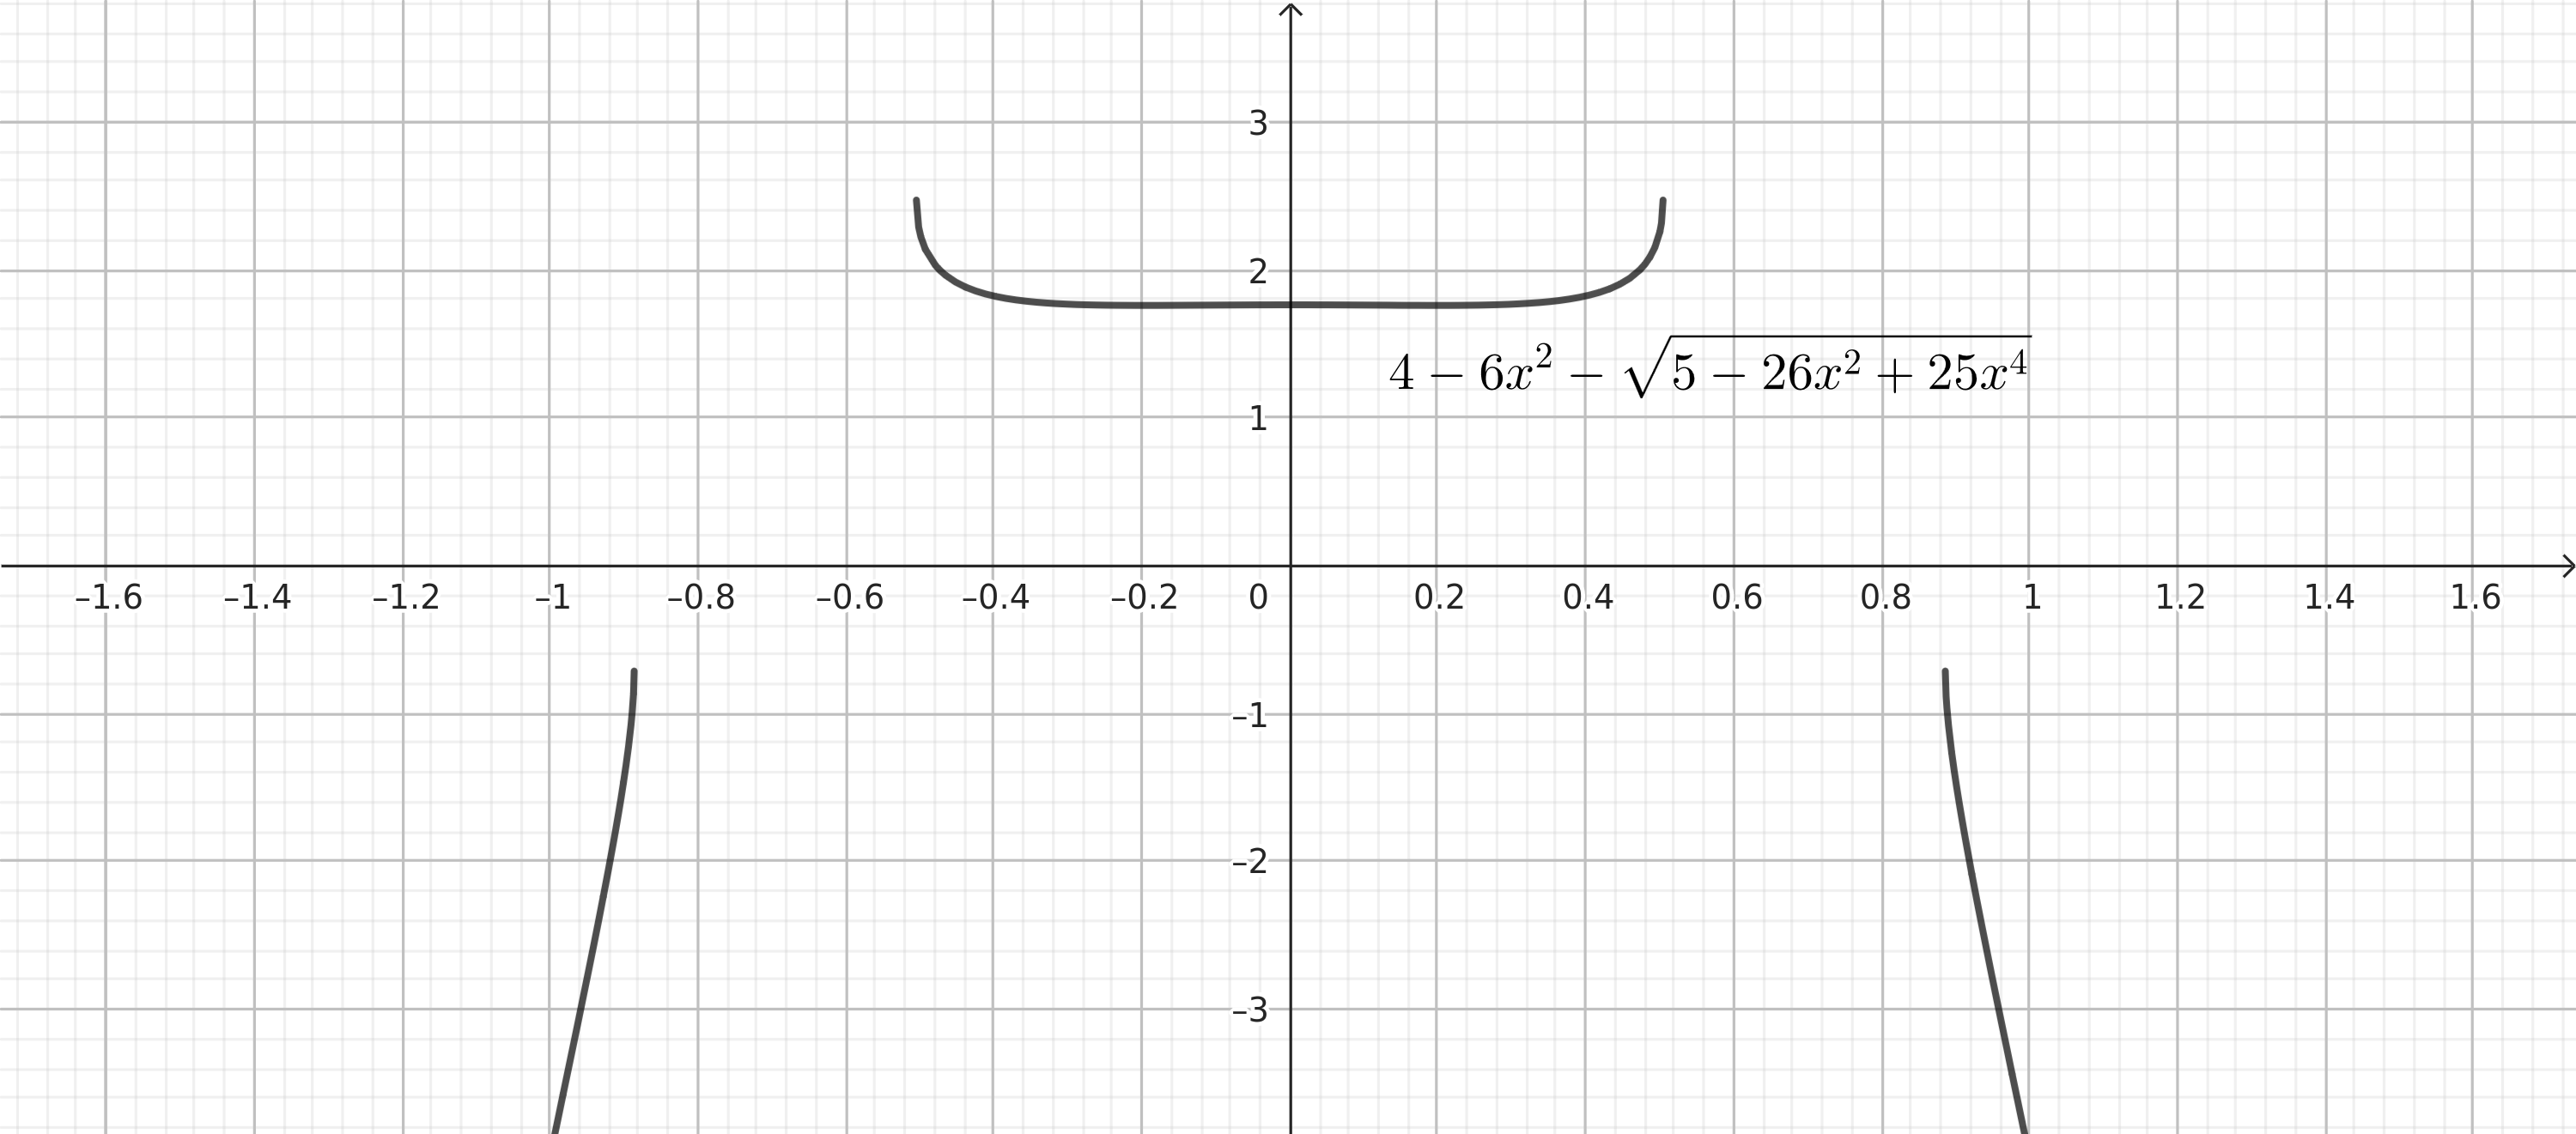
\includegraphics[width=0.7\textwidth]{geogebra_sqrt.png}
  \end{center}
  This shows us, that when $a$ lies between $-0.51$ and $0.51$, the polynomial above has a solution in the real plane. By looking at the other branches of the solution, we see that there is also an isolated solution in $a = 1$, $b = 0$ corresponding to the degenerate triangle. However, this solution is excluded by the conditions on the segment. For other values of $a$ there is no solution over the reals.

  By doing a bit of manual analysis and plotting parts of the graph seperately, the complete set of solutions in the real plane can be found on figure~\ref{fig:orthic_wow}. The two blobs are solutions for acute triangles, whereas the the two unbounded curves correspond to solutions for obtuse triangles.

  We're lucky in this case, as the quartic is solvable in radicals. Had the pseudo-remainder been of fifth degree (ignoring the factors from the conditions on the segment), we might not be able to say much about the real case. Hence this method of discovering geometric theorems may not always work in the real plane. It could, however, be a useful first step, as we do get nescesary and sufficient conditions for the theorem to be true. Those conditions just might be difficult to analyse, but more sophisticated tools can use this as a first step, see \cite{10.1145/2755996.2756646}.

  % Further experimentation reveals, that for acute triangles, the the area of the orthic triangle can reach a maximum of one fourth of $A_{ABC}$. For obtuse triangles, it seems like the orthic triangle can get almost twice as big as $ABC$, but not quite. This also highlights another limitation of this approach, that we're only able to answer questions, which can be encoded as a polynomial. Determining which triangles has be largest ratio between the areas of the triangle and its orthic triangle is not possible with this technique. Although, using numeric optimization techniques, one could get reasonable answer.
\end{example}

\begin{figure}[t]
  \begin{center}
    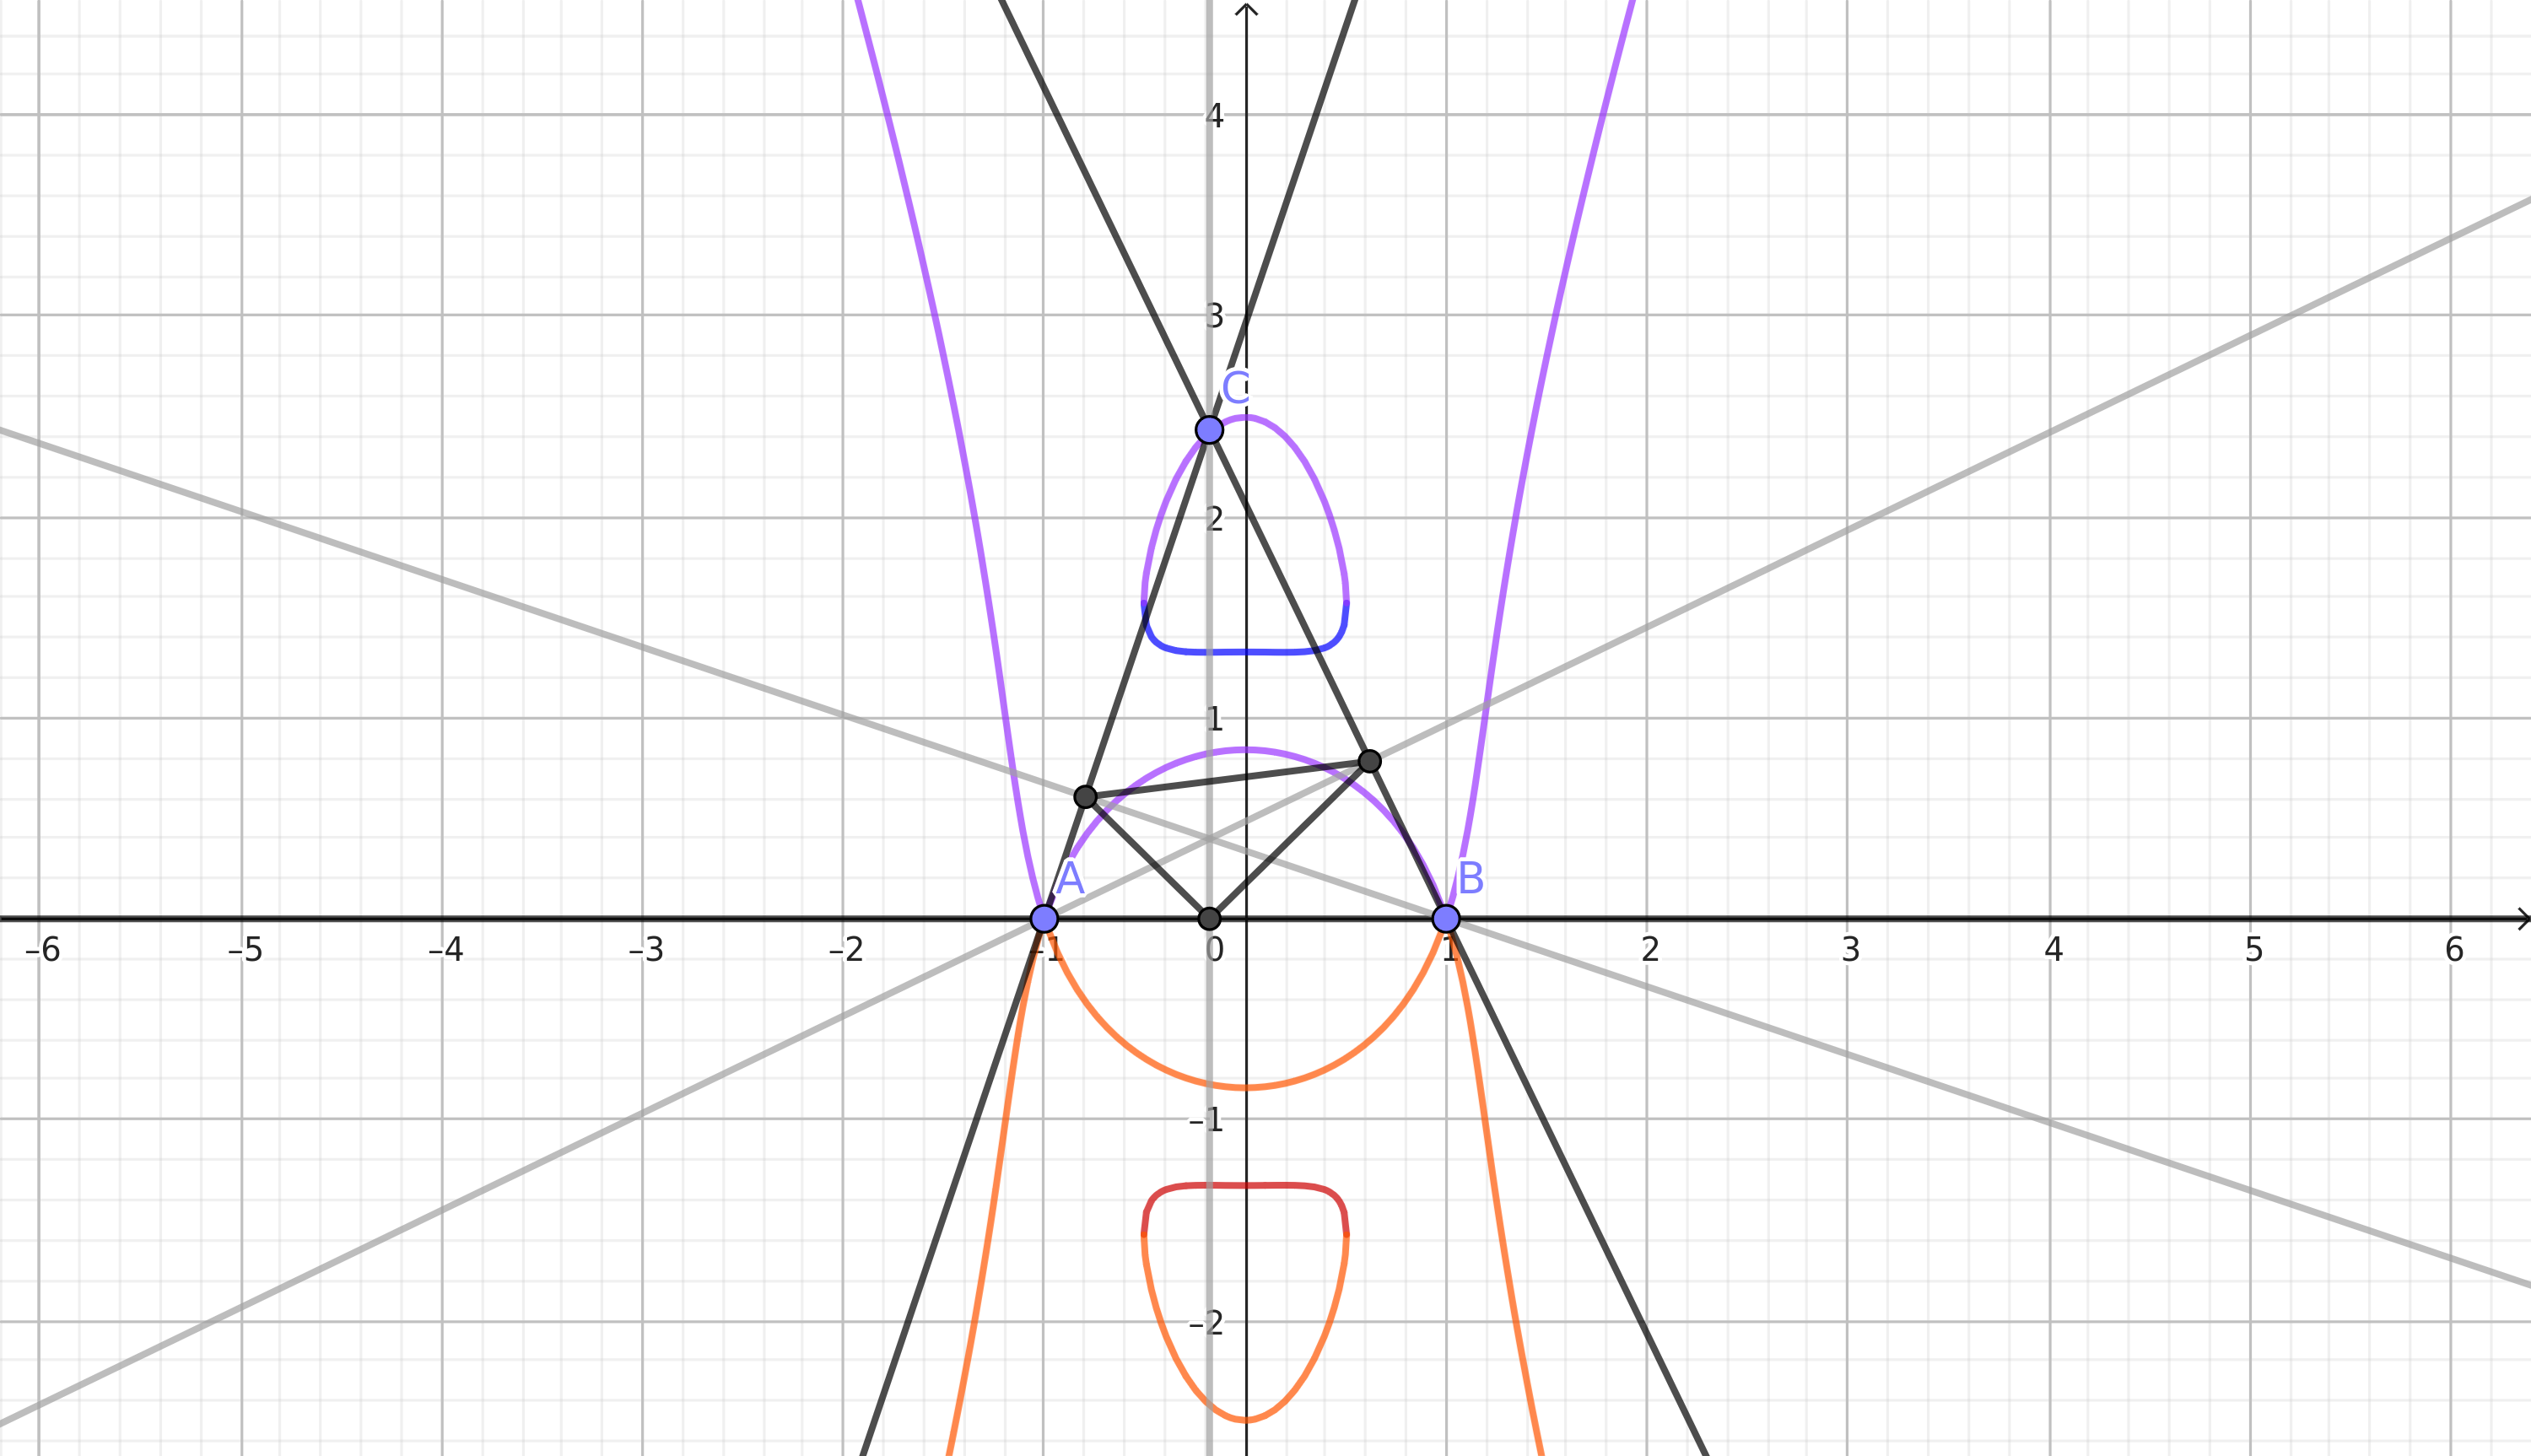
\includegraphics[width=0.7\textwidth]{geogebra_orthic_wow.png}
  \end{center}
  \caption{The set of real points, where the area of the orthic triangle is exactly one fifth of the area of the triangle $ABC$} \label{fig:orthic_wow}
\end{figure}










\subsection[Bernds conjecture]{Bernds conjecture\footnote{Named such by Bernd Sturmfels in a private communication to the supervisor of this project.}}\label{sec:bernd}
In the article~\cite{sturmfels}, Bernd Sturmfels states the following theorem without proof.

\begin{theorem}
  Let $K$ be an algebraically closed field and $F = \{f_{1}, \dots, f_{k}\} \subset K[x_{1}, \dots, x_{n}]$ a finite set of polynomials. Assume that $\,\V(F) = \emptyset$ and consider the ideal $\,I = \langle y_{1} - f_{1}, \dots, y_{k} - f_{k} \rangle \subset K[x_{1}, \dots, x_{n}, y_{1}, \dots, y_{k}]$. Let $G$ be a Gröbner basis of $\,I$ with respect to the lexicographic order with $x_{1} > \dots > x_{n} > y_{1} > \dots > y_{k}$. Then $G$ contains a polynomial $p$ (called a final polynomial) such that
  \begin{enumerate}
    \item $p(x_{1}, \dots, x_{n}, 0, 0, \dots, 0) \in K \setminus \{0\}$
    \item $p(x_{1}, \dots, x_{n}, f_{1}, \dots, f_{k}) = 0$.
  \end{enumerate}
\end{theorem}

He writes that the proof is ``straightforward but fairly technical''. In a private communication\cite{NL_to_BS} with Sturmfels, he encourages us to write a proof or find a counterexample. He also writes, that the gist of the argument he had in mind was using specializations of Gröbner bases. Since since $\{x_{1}, \dots, x_{n}\} \gg \{y_{1}, \dots, y_{k}\}$, the Gröbner basis of $I$ would specialize to a Gröbner basis of $\langle F \rangle$ when we specialize the $y_{i}$'s to zero. However, as we have seen, Gröbner bases can be most unstable under specializations. Indeed, the following counterexample disproves this line of reasoning and the theorem.

\begin{example}\upshape
  Let $F = \{f_{1}, f_{2}\}$ where $f_{1} = x_{1} x_{2} + 1$ and $f_{2} = x_{2}$. Then, the corresponding ideal
  $I = \langle y_{1} - f_{1}, y_{2} - f_{2} \rangle$ has the following reduced Gröbner basis w.r.t. the lexicographic order with $x_{1} > x_{2} > y_{1} > y_{2}$: $G =  \{g_{1}, g_{2}\}$ where $g_{1} = x_{2} - y_{2}$ and $ g_{2} = y_{2}x_{1} - y_{1} + 1$. Consider now $G' = \{g_{1}, g_{1} - g_{2}\} = \{x_{2} - y_{2}, y_{2}x_{1} + x_{2} - y_{1} - y_{2} + 1\}$. Clearly $\langle G' \rangle = \langle G \rangle = I$, and it is still a Gröbner basis since $\LT(G') = \LT(G)$. However, letting $\sigma$ be the specialization setting $\sigma(y_{1}) = \sigma(y_{2}) = 0$, we see that
  \[\sigma(G') = \{x_{2}, 1+x_{2}\}\]
  which is not a Gröbner basis. Furthermore, we see that $G'$ does not contain a final polynomial.
\end{example}

While this example is admittedly a bit contrived, the theorem if false, even if we require the Gröbner basis to be reduced.

\begin{example}\upshape
    Let $F = \{f_1, f_2, f_3\}$ where $f_1 = x_2 + x_3$, $f_2 = x_2 x_3$ and $f_3 = x_1 x_3 + 1$. The reduced Gröbner basis of $\langle F \rangle$ is $\{1\}$, so $F$ has no common zeros. The corresponding ideal $I = \langle y_1 - f_1, y_2 - f_2, y_3 - f_3 \rangle$ has the reduced Gröbner basis
    \begin{gather*}
    G = \{ x_3^2 - x_3 y_1 + y_2, x_2 + x_3 - y_1, x_1 y_2 + x_3 y_3 - x_3 - y_1 y_3 + y_1, x_1 x_3 - y_3 + 1\}.
    \end{gather*}
    When specializing $y_1 = y_2 = y_3 = 0$, $G$ turns into
    \[\bar G = \{ x_3^2, x_2 + x_3, -x_3, x_1 x_3 + 1\}\]
    which is not a Gröbner basis, and does not contain a constant. Hence, $G$ does not contain a final polynomial.
\end{example}

To fix the theorem, we can turn to parametric Gröbner bases. To shorten notation, let $X = \{x_{1}, \dots, x_{n}\}$ and $Y = \{y_{1}, \dots, y_{k}\}$.

\begin{theorem}
  Let $K$ be an algebraically closed field and let $F = \{f_{1}, \dots, f_{k}\} \subset K[X]$ be a finite set of polynomials. Assume that $\V(F) = \emptyset$ and consider the ideal $I = \langle y_{1} - f_{1}, \dots, y_{k} - f_{k} \rangle \subset K[X, Y]$. Let $G$ be a comprehensive parametric Gröbner basis of $\,I$ with respect to the lexicographic order with $x_{1} > \dots > x_{n} > y_{1} > \dots > y_{k}$. Then $G$ contains a final polynomial.
\end{theorem}
\begin{proof}
  First, notice that every polynomial in $I$ satisfies the second property of final polynomials, since the generators does, and the evaluation map is linear. Thus, we only need to prove that a parametric Gröbner basis contains an element satisfying the first property.

  Let $G$ be a parametric Gröbner basis of $I$, and let $\sigma$ be the specialization setting $\sigma(y_{i}) = 0$ for every $i$. Since $\langle \sigma(I) \rangle = \langle F \rangle = \langle 1 \rangle$, there must be some element $g \in G$ where $\LM(\sigma(g)) \mid 1$, implying that $g$ is a final polynomial.
\end{proof}

However, parametric Gröbner bases can be quite expensive to compute since we need to repeatedly compute Gröbner bases, and furthermore we don't have nice bounds on the degrees. But we only care about one single specialization. This means we don't need a parametric Gröbner basis, we just need a faithful segment of a Gröbner system covering the origin. Here, we can use lemma~\ref{lem:grb_if_nmap_to_z_t}. Let $\sigma^{1} : K[t, X, Y] \to K[X, Y]$ be the map evaluating $t$ to 1, and let $\sigma^{0} : K[t, X, Y] \to K[X, Y]$ be the map evaluating $t$ to 0.

\begin{theorem}
  Let $K$ be an algebraically closed field and $F = \{f_{1}, \dots, f_{k}\} \subset K[X]$ a finite set of polynomials. Assume that $\V(F) = \emptyset$ and consider the ideal $I = \langle \hat F \rangle$ where $\hat F = \{y_{1} - f_{1}, \dots, y_{k} - f_{k}\}$. Now, let $\,G$ be the reduced Gröbner basis of the ideal $\langle t \cdot \hat F \cup (1 - t) \cdot Y \rangle \subset K[t, X, Y]$ w.r.t.\ any monomial order with $t \gg X \gg Y$. Then $\sigma^{1}(G)$ contains a final polynomial.
\end{theorem}
\begin{proof}
  As before, we only need to show that $\sigma^{1}(G)$ contains a polynomial satisfying the first property of final polynomials. Let $\sigma : K[X, Y] \to K[X]$ be the specialization setting $\sigma(y_{i}) = 0$ for every $i$ and let $H = \{\LC_{Y}(g) \mid g \in G, \LT(g) \notin K[X, Y], \LC_{X, Y}(g) \notin \langle Y \rangle\}$. If we have $0 \in \V(Y) \setminus \V(\lcm(H))$, then lemma~\ref{lem:grb_if_nmap_to_z_t} gives us that $\sigma(\sigma^{1}(G))$ is a Gröbner basis of $\langle \sigma(I) \rangle = \langle F \rangle$. By the Nullstellensatz, $\langle F \rangle = \langle 1 \rangle$, so $\sigma(\sigma^{1}(G))$ has to contain a constant. This implies, that $\sigma^{1}(G)$ contains a final polynomial $g$.

  Now, we just need that $0 \in \V(Y) \setminus \V(\lcm(H))$. Since $\V(Y) = \{0\}$, we just need that $\V(Y) \nsubset \V(\lcm(H))$. By lemma~\ref{lem:LC_U_notin_S} we have that $h \notin \langle Y \rangle$ for each $h \in H$. Since $\langle Y \rangle$ is a prime ideal, this implies that $\lcm(H) \notin \langle S \rangle$. Thus $\V(Y) \nsubset \V(\lcm(H))$.
\end{proof}

This counterexample and theorem was developed in colaboration with Peter Lundgaard, and resulted in an article \cite{Lundgaard_Poulsen}. In that article, it is also proven that it is enough to compute a Gröbner basis of $\langle y_{1} - z f_{1}, \dots, y_{k} - z f_{k} \rangle$. However, that proof requires a little more care, whereas this proof follows directly from the theory of parametric Gröbner bases.
